\chapter{Experimentación}

En este capítulo se van a exponer todas las pruebas realizadas sobre los \textit{scripts} de entrenamiento. Estas pruebas van desde \textit{profiling} de memoria hasta la prueba de entrenamiento de los modelos usando distintos hiperparámetros. De estos últimos se realizará un análisis para conocer bien cuáles son los hiperparámetros que más influencia tienen sobre la métrica que mide la capacidad de clasificación del modelo generado.\\

Además de lo anterior, se realizará una comparación entre los mejores resultados obtenidos en cada experimento y una comparación del uso de memoria.\\

Me gustaría también agradecer a las personas del \textit{Southern Wide-field Gamma-ray Observatory} (\textit{SWGO}) y del \textit{Laboratório de Instrumentação e Física Experimental de Partículas} (\textit{LIP}), más concretamente a Mario Pimenta, Ruben Conceição y Bernardo Tomé, por proveerme del conjunto de datos obtenido de sus simulaciones. Un análisis de estos datos se encuentra en la Seccción \ref{chap:datanalysis}.

\section{Memory profiling}

En esta sección, mostraré los resultados del \textit{profiling} de memoria realizado a todos los scripts de entrenamiento para saber cuánta memoria usan y por tanto es necesaria para poder ejecutarlos.\\

El \textit{profiling} nos permite conocer los recursos que un \textit{software} (en este caso los \textit{script}) necesita. Hoy en día tenemos la suerte de que los componentes de un computador decente está al alcance de casi todos (excepto las \textit{GPU}s cuando hay un \textit{boom} de criptomonedas). Pero si los componentes son accesibles económicamente para casi todo el mundo, ¿para qué hacemos \textit{profiling} entonces? Vamos a imaginar que queremos montar un computador de alto rendimiento para entrenar modelos lo más rápido posible. Tal vez la inversión más importante sea una buena \textit{GPU} por el tema de aprovechar el paralelismo que ofrece. Y ahora viene otra pregunta ¿cuánta \textit{RAM} necesitamos? Si ponemos demasiada sería un poco derroche económico pero si nos quedamos cortos se usaría memoria alocada en el disco duro (\textit{SWAP}) que es mucho más lenta que la \textit{RAM} y por tanto ralentizaría nuestras ejecuciones. Si sabemos la cantidad de \textit{RAM} que consumen nuestros \textit{scripts} o \textit{software} podemos conocer la cantidad de memoria que vamos a necesitar en nuestro computador.\\

También sería conveniente analizar cuanta memoria usa nuestro modelo una vez desplegado de nuevo para hacer la inversión correcta en memoria \textit{RAM}. Pero la cosa no queda ahí, ¿Y si queremos desplegar nuestro modelo en un dispositivo empotrado\footnote{Los dispositivos empotrados (como por ejemplo \textit{Arduino}, \textit{ESP32} o \textit{ARM}) normalmente tienen recursos muy limitados (suelen tener por lo general unos pocos KiBs o MiBs de RAM) y poco uso de energía, pues suelen funcionar con baterías y nos interesa que estas duren lo máximo posible.}? En este caso nos estamos refiriendo al campo del \textit{tinyML}. Estos dispositivos no suelen tener una gran cantidad de memoria (no suelen llegar ni al medio GiB) por tanto en estos casos también nos interesa usar \textit{profiling} e intentar optimizar lo máximo posible el uso de memoria y \textit{CPU}\footnote{En el caso del \textit{tinyML} también sería interesante el uso de un \textit{profiler} de \textit{CPU}.} para ahorrar la máxima batería posible. Para este caso de uso existen librerías de \textit{Machine Learning} más ligeras como \textit{PyTorch Lite} o \textit{TensorFlow Lite}.\\

Ya hemos hablado del \textit{tinyML}, pero ¿sería interesante también tener en cuenta el uso de memoria en el contexto de \textit{Edge Computing}? En este caso, tendríamos sensores que publican datos en \textit{streaming} o publican estados de algún objeto en tiempo real y un computador que se subscribe a los datos para analizarlos en tiempo real o enviarlos a la \textit{cloud} de una gran empresa para usarlos en futuras mejoras del sistema. Estos sensores y dicho computador tal vez están manejando un vehículo autónomo con una familia dentro. Si dicho computador que controla el vehículo se queda corto de memoria podría dejar de responder a los estímulos externos en tiempo real y producirse una catástrofe. Con esto quiero recalcar que es esencial el uso de \textit{profiling} en sistemas críticos.\\

En conclusión, en estos párrafos anteriores se deja demostrada la importancia del \textit{profiling} a la hora de diseñar sistemas que vayamos a desplegar en algún dispositivo ya sea empotrado o no y la esencialidad del mismo a la hora del diseño de sistemas críticos que puedan llevar a la pérdida de vidas humanas.\\

\subsection{Memory profiling para \textit{Convolutional Autoencoder}}

El modelo que ha sido perfilado en esta sección ha sido descrito en la Sección \ref{subsec:cae}.

\begin{figure}[H]
	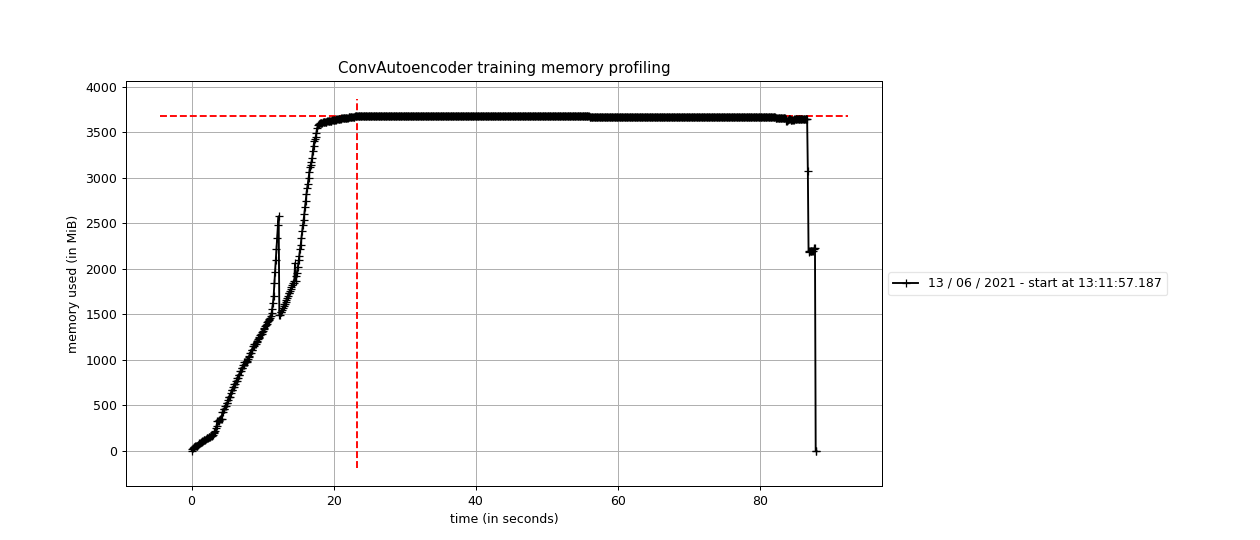
\includegraphics[width=1.\linewidth]{imagenes/06_Experimentacion/cae.png}
	\centering
	\caption{Gráfico de uso de memoria del script de entrenamiento de entrenamiento para el ConvAutoencoder (\path{src/cae.py}).}
\end{figure}

Al principio, puede observarse una subida muy pronunciada debido a la lectura del dataset (ocupa aproximadamente 1500 MiB en memoria). A parte, también se puede observar otra gran subida producida al cargar el modelo de \textit{Machine Learning} en la GPU. El uso total de memoria de este script es de 3650.3 MiB, aproximadamente 3.56 GiB.\\

\subsection{Memory profiling para \textit{Convolutional Classifier}}

El modelo que ha sido perfilado en esta sección ha sido descrito en la Sección \ref{subsec:convnet}.

\begin{figure}[H]
	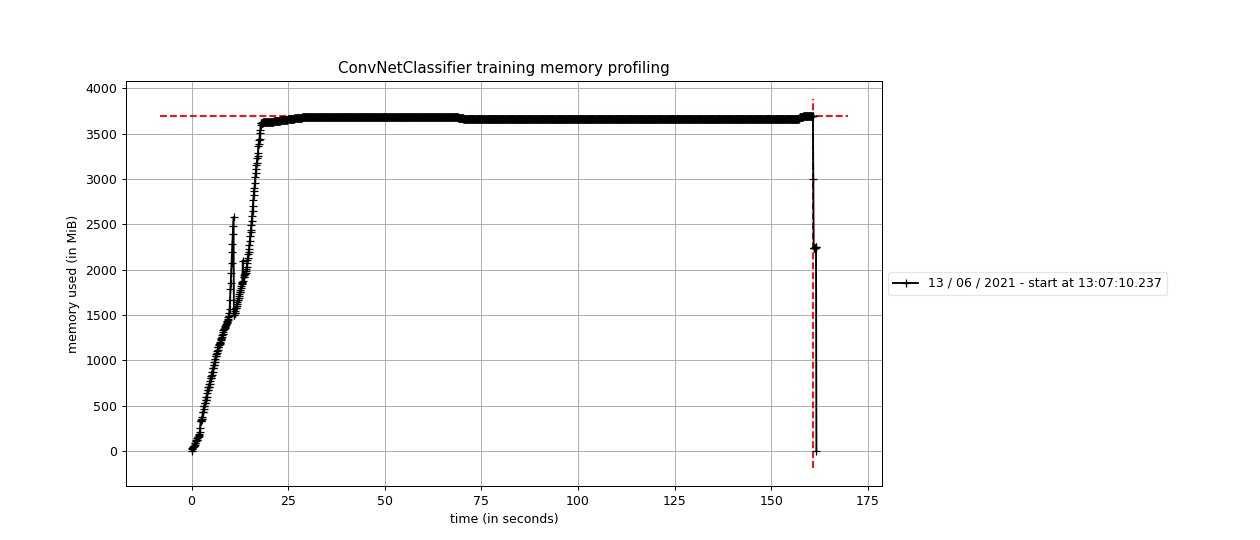
\includegraphics[width=1.\linewidth]{imagenes/06_Experimentacion/convnet.png}
	\centering
	\caption{Gráfico de uso de memoria del script de entrenamiento de entrenamiento para el ConvClassifier (\path{src/convnet.py}).}
\end{figure}

El máximo de memoria requerida durante la ejecución del script de entrenamiento es de 3693.7 MiB, aproximadamente 3.61GiB. En este caso, las subidas son debidas a la lectura del dataset y a la carga del modelo en la GPU.\\

\subsection{Memory profiling para \textit{ResNet}}

El modelo que ha sido perfilado en esta sección está descrito en la anterior Sección \ref{subsec:resnet}.

\begin{figure}[H]
	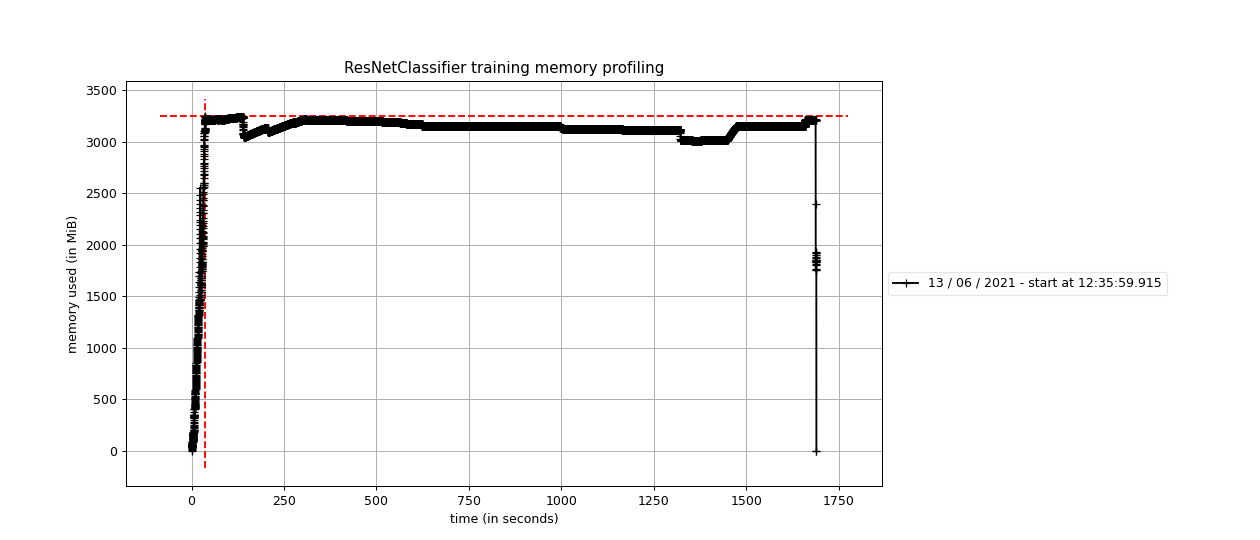
\includegraphics[width=1.\linewidth]{imagenes/06_Experimentacion/resnet.png}
	\centering
	\caption{Gráfico de uso de memoria del script de entrenamiento de entrenamiento para el ResNetModel (\path{src/resnet.py}).}
\end{figure}

Este script requiere menos memoria para poder ejecutarse en condiciones que los demás, pues requiere 3214.6 MiB, aproximadamente 3.14 GiB. El incremento de uso en memoria es debido a, como en las Subsecciones anteriores, la carga del dataset y la carga del modelo en GPU.\\

\subsection{Memory profiling para \textit{Varitional Autoencoder}}

El modelo que ha sido perfilado en esta sección está descrito en la anterior Sección \ref{subsec:vae}.

\begin{figure}[H]
	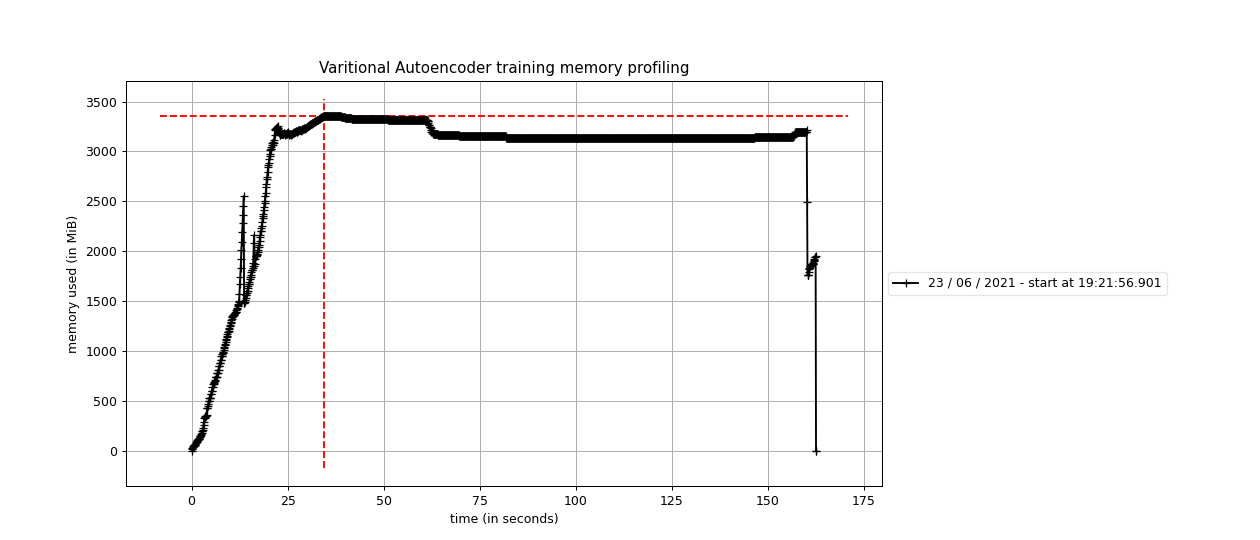
\includegraphics[width=1.\linewidth]{imagenes/06_Experimentacion/vae.png}
	\centering
	\caption{Gráfico de uso de memoria del script de entrenamiento de entrenamiento para el Varitional Autoencoder (\path{src/vae.py}).}
\end{figure}

El script de entrenamiento del Varitional Autoencoder requiere 3223.1 MiB de memoria, aproximadamente 3.15 GiB. Las partes del script que más han incrementado el uso de memoria coincide con los otros experimentos que han sido perfilados en las Subsecciones anteriores.\\

\subsection{Comparativa final del uso de memoria}

\begin{table}[H]
\centering
\begin{tabular}{cc}
\hline
\textbf{Script}                    & \textbf{Uso de memoria} \\ \hline
\path{src/cae.py}                  & 3.56 GiB                \\ \hline
\path{src/convnet.py}              & 3.61 GiB                \\ \hline
\path{src/resnet.py}               & 3.14 GiB                \\ \hline
\path{src/vae.py}                  & 3.15 GiB                \\ \hline
\end{tabular}
\caption{Resultados globales del \textit{profiling} de memoria.}
\label{tab:memoryprofile}
\end{table}

Como se puede ver en la Tabla \ref{tab:memoryprofile}, el script que más memoria consume es el que se encuentra en \path{src/convnet.py}, pero el que se encuentra en \path{src/cae.py} consume casi lo mismo. Los otros dos scripts consumen en torno a los 3.15 GiB. El tamaño de memoria que le pondría a una máquina de entrenamiento para este conjunto de datos sería de un mínimo de 8GiB\footnote{Usando dos módulos de 4 GiB idénticos para aprovechar las ventajas del \textit{Dual Channel}.}, pues hay que dejar espacio para las rutinas del SO y con 4GiB se quedaría corto.

\section{Configuración de las pruebas de diseño}

En esta Sección se va a presentar la configuración de todos los experimentos implementados y el rango de valores que puede tomar sus hiperparámetros junto con la distribución de los mismos.\\

\subsection{Configuración común entre experimentos}

\textit{SnapperML} no permite establecer un fichero de configuración con variables globales, lo que me refiero en esta Subsección con configuración global es a variables que he usado en todos los experimentos con los mismos valores.\\

\setlength{\tabcolsep}{10pt} % Default value: 6pt
\renewcommand{\arraystretch}{1.5} % Default value: 1

\begin{table}[h]
\centering
\begin{tabular}[c]{m{3cm}m{3cm}}
\hline
\textbf{Variable} & \textbf{Valor} \\ \hline
epochs            & 5              \\
seed              & 2342           \\ \hline
\end{tabular}
\caption{Configuración global para todos los experimentos.}
\label{tab:globalvalues}
\end{table}

En la Tabla \ref{tab:globalvalues} quiero decir que todos los modelos creados en los experimentos se entrenan durante 5 épocas (entendidas estas como un pase completo por todos los \textit{batches} del conjunto de datos) y se inicializa el generador aleatorio de \textit{PyTorch} con la semilla 2342. Aunque 5 épocas parezca poco, ya se pueden obtener buenos resultados (véase Tabla \ref{tab:results}).

\subsection{Configuración \textit{Convolutional Autoencoder}}

Los hiperparámetros de este modelo han sido exlicados en la Subsección \ref{subsec:cae}. En este experimento, se usa el modelo introducido en la Subsección \ref{subsub:convautoencoder}. Con este modelo se puede realizar una reducción de dimensionalidad de los datos para aprender de datos simplificados en lugar de los originales. Por esa razón es un modelo interesante para experimentar.\\

\begin{table}[H]
\centering
\begin{tabular}[c]{m{6cm}m{3cm}}
\hline
\textbf{Variable}                 & \textbf{Valor}  \\ \hline
Nombre del experimento            & CAE             \\
Número de configuraciones         & 1               \\ \hline
\end{tabular}
\caption{Información general sobre el experimento \textit{Convolutional Autoencoder}.}
\label{tab:caeinfo}
\end{table}

\begin{table}[H]
\centering
\begin{tabular}{m{4cm}m{5.1cm}}
\hline
\textbf{Variable}                 & \textbf{Valor}                          \\ \hline
\textit{Batch Size}               & randint(32,256)                         \\
\textit{Learning rate}            & loguniform(0.0001, 0.01)                \\
\textit{Regularization}           & loguniform(0.0001, 0.1)                 \\
Canales de salida en la primera convolución &   randint(1, 10)              \\
Profundidad                       & randint(1,4)                            \\
Tamaño del código latente         & randint(10, 100)                        \\
Optimizador                       & choice(['adam', 'sgd'])                 \\ \hline
\end{tabular}
\caption{Hiperparámetros para el experimento \textit{Convolutional Autoencoder}.}
\label{tab:caeconfig}
\end{table}

En este y en todos los siguientes experimentos se ha probado con un \textit{batch size} variable para ver si afecta al resultado final o no. Además, también se ha probado con un \textit{learning rate} y con un valor de regularización que toman valores en un rango amplio. También pruebo con dos optimizadores para compararlos, \textit{Adam} (explicado en la Subsección \ref{subsec:learningalgorithms}) y \textit{SGD} (explicado en la misma Subsección).\\

Además, he experimentado con varios valores para el número de canales de salida en la primera convolución (tomando valores entre 1 y 10), con varios valores para la profundidad del \textit{encoder} y del \textit{decoder} (de 2 a 4, pues si toma un valor mayor el tamaño de la imagen sería aproximadamente de 2x2 y se usan \textit{kernels} de 3x3 en las operaciones convolucionales). Por último, he probado también con varios valores para el tamaño del código latente (de 10 a 100).\\

\subsection{Configuración \textit{Convolutional Classifier}}

Los hiperparámetros de este modelo han sido exlicados en la Subsección \ref{subsec:convnet}. En resumen a dicha Subsección, en este experimento se prueba con una red convolucional basasda en \textit{LeNet-5} (un modelo bastante simple pero con buenos resultados) con un número de canales de salida variable para cada convolución para que con \textit{optuna} se encuentre la mejor combinación posible que maximice la métrica objetivo.\\

\begin{table}[H]
\centering
\begin{tabular}[c]{m{6cm}m{3cm}}
\hline
\textbf{Variable}                 & \textbf{Valor}  \\ \hline
Nombre del experimento            & Simple CNN      \\
Número de configuraciones         & 1               \\ \hline
\end{tabular}
\caption{Información general sobre el experimento \textit{Convolutional Classifier}.}
\label{tab:convnetinfo}
\end{table}

\begin{table}[H]
\centering
\begin{tabular}{m{3cm}m{5.1cm}}
\hline
\textbf{Variable}                 & \textbf{Valor}                          \\ \hline
\textit{Batch Size}               & randint(32,256)                         \\
\textit{Learning rate}            & loguniform(0.0001, 0.01)                \\
Optimizador                       & choice(['adam', 'sgd'])                 \\ 
Output channels                   & randint(2, 20) $\times$ randint(2, 20)  \\ \hline
\end{tabular}
\caption{Hiperparámetros para el experimento \textit{Convolutional Classifier}.}
\label{tab:convnetconfig}
\end{table}

La última diferencia que tiene este experimento con el anterior es que se genera una \textit{List} aleatoria para probar con distintos valores de canales de salida de las capas convolucionales y ver como afecta a las métricas.\\

\subsection{Configuración \textit{ResNet}}\label{subsec:resnet}

Los hiperparámetros de este modelo han sido exlicados en la Subsección \ref{subsec:resnetarch}. En resumen a dicha Subsección, se va a usar una implementación basada en \textit{ResNet}, una red convolucional muy popular en el campo de clasificación de imágenes y por tanto con una gran capacidad de clasificación (tal vez de las mejores). Este caso particular de \textit{ResNet} tiene un número de canales para cada grupo de \textit{ResBlocks} variable y el número de \textit{ResBlocks} en cada grupo también es variable.\\

\begin{table}[H]
\centering
\begin{tabular}[c]{m{6cm}m{3cm}}
\hline
\textbf{Variable}                 & \textbf{Valor}  \\ \hline
Nombre del experimento            & ResNet          \\
Número de configuraciones         & 1               \\ \hline
\end{tabular}
\caption{Información general sobre el experimento \textit{ResNet}.}
\label{tab:resnetinfo}
\end{table}

\begin{table}[H]
\centering
\begin{tabular}{m{3cm}m{7cm}}
\hline
\textbf{Variable}                 & \textbf{Valor}                          \\ \hline
\textit{Batch Size}               & randint(32,256)                         \\
\textit{Learning rate}            & loguniform(0.0001, 0.01)                \\
\textit{Regularization}           & loguniform(0.0001, 0.1)                 \\
Optimizador                       & choice(['adam', 'sgd'])                 \\ 
Número de bloques                 & randint(2, 6) $\times$ randint(2, 6) $\times$ randint(2, 6) $\times$ randint(2, 6) \\
Número de canales                 & randint(8, 32) $\times$ randint(32, 64) $\times$ randint(64, 128) $\times$ randint(128, 256) $\times$ randint(256, 512) \\
\hline
\end{tabular}
\caption{Hiperparámetros para el experimento \textit{ResNet}.}
\label{tab:resnetconfig}
\end{table}

El número de bloques toma un valor entre 2 y 6 porque tampoco quiero que el modelo sea muy profundo (y por tanto tarde demasiado tiempo en ajustarse a los datos de entrenamiento). El número de canales va aumentando conforme vamos profundizando en la red, tal y como sucede en el modelo original.

\subsection{Configuración \textit{Varitional Autoencoder}}

Los hiperparámetros de este modelo han sido exlicados en la Subsección \ref{subsec:vae}. Este modelo no usa ninguna capa convolucional y por eso mismo es interesante experimentar con él, para compararlo con otros modelos convolucionales. Como se ha especificado en la Subsección de antes, este modelo tiene el número de neuronas por capa variable, permitiendo a \textit{optuna} encontrar aquel que maximice la métrica objetivo.\\

\begin{table}[H]
\centering
\begin{tabular}[c]{m{6cm}m{3cm}}
\hline
\textbf{Variable}                 & \textbf{Valor}  \\ \hline
Nombre del experimento            & ResNet          \\
Número de configuraciones         & 1               \\ \hline
\end{tabular}
\caption{Información general sobre el experimento \textit{Varitional Autoencoder}.}
\label{tab:resnetinfo}
\end{table}

\begin{table}[H]
\centering
\begin{tabular}{m{3cm}m{7cm}}
\hline
\textbf{Variable}                 & \textbf{Valor}                          \\ \hline
\textit{Batch Size}               & randint(32,256)                         \\
\textit{Learning rate}            & loguniform(0.0001, 0.01)                \\
\textit{Regularization}           & loguniform(0.0001, 0.1)                 \\
Optimizador                       & choice(['adam', 'sgd'])                 \\ 
Tamaño de las capas               & randint(500, 1000) $\times$ randint(100, 500) $\times$ randint(50, 100) $\times$ randint(10, 50) \\
\hline
\end{tabular}
\caption{Hiperparámetros para el experimento \textit{Varitional Autoencoder}.}
\label{tab:resnetconfig}
\end{table}

\section{Resultados}

En esta sección se presentan los resultados obtenidos de la ejecución de los experimentos anteriores. La métrica usada para seleccionar al mejor ha sido la \textit{$F_1$ score}. Para calcular esta métrica, se hace uso de otras dos, la \textit{precision} y el \textit{recall}.\\

En una clasificación binaria, podemos clasificar las predicciones tal que así:

\begin{table}[H]
\centering
\begin{tabular}{c|c|c|}
\cline{2-3}
 &
  \textbf{\begin{tabular}[c]{@{}c@{}}Predicción\\ Positivo\\ (y=1)\end{tabular}} &
  \textbf{\begin{tabular}[c]{@{}c@{}}Predicción\\ Negativo\\ (y=0)\end{tabular}} \\ \hline
\multicolumn{1}{|c|}{\textbf{\begin{tabular}[c]{@{}c@{}}Positivo\\ (y=1)\end{tabular}}} &
  \begin{tabular}[c]{@{}c@{}}Verdaderos\\ Positivos\end{tabular} &
  \begin{tabular}[c]{@{}c@{}}Falsos\\ Negativos\end{tabular} \\ \hline
\multicolumn{1}{|c|}{\textbf{\begin{tabular}[c]{@{}c@{}}Negativo\\ (y=0)\end{tabular}}} &
  \begin{tabular}[c]{@{}c@{}}Falsos\\ Positivos\end{tabular} &
  \begin{tabular}[c]{@{}c@{}}Verdaderos\\ Negativos\end{tabular} \\ \hline
\end{tabular}
\caption{Clasificación de las predicciones.}
\label{tab:predictions}
\end{table}

\begin{align}
	&Precision = \frac{True Positives}{True Positives + False Positives}\\
	&Recall = \frac{True Positives}{True Positives + False Negatives}
\end{align}

Por tanto, la \textit{precision} mide el balance entre los verdaderos positivos y lo que se predice como positivo (ya sea verdadero o falso). Por otra parte, el \textit{recall} mide el balance entre los verdaderos positivos y los positivos que han sido predecidos bien o mal. Una vez que ya sabemos como se calcula la \textit{precision} y el \textit{recall}, podemos calcular la \textit{$F_1$ score} de la forma siguiente:

\begin{align}
&F_1 score = 2 \frac{precision \cdot recall}{precision + recall}
\end{align}

En la Tabla \ref{tab:results} se muestran los resultados de los experimentos (los mejores modelos obtenidos de cada uno) y en la Figura \ref{fig:confusion} se muestran las \textit{confusion matrices} de los resultados. Como se puede observar, los resultados no son muy distintos de un experimento a otro, pues todos tienen casi el mismo \textit{$F_1$ score}. El modelo que tiene menor valor en esta métrica es el \textit{Varitional Autoencoder}, los modelos con capas convolucionales tienen mejores resultados que este último. El experimento que mejor resultado ha tenido, aunque tampoco hay mucha diferencia, ha sido el de \textit{Simple CNN} (modelo basado en LeNet-5). En las \textit{Confusion matrices} se puede observar que no hay mucha diferencia entre una y otra, pues en todos los casos son capaces de predecir bien cerca del 99\% de las muestras.\\

\begin{figure}[H]
\begin{subfigure}{.5\textwidth}
  \centering
  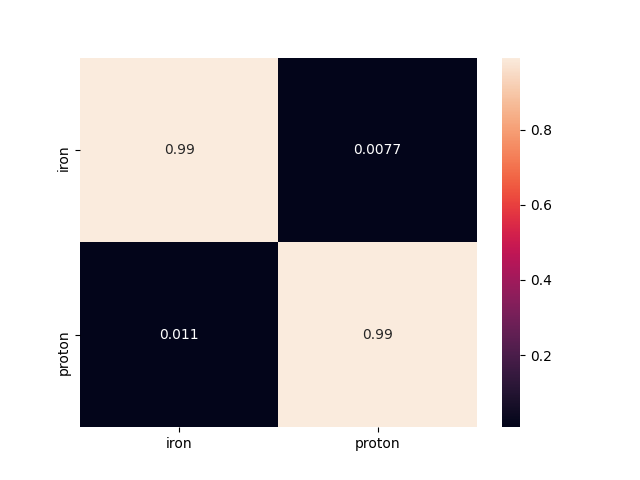
\includegraphics[width=.8\linewidth]{imagenes/06_Experimentacion/simplecnncm.png}  
  \caption{Simple CNN confusion matrix.}
  \label{fig:simplecnncm}
\end{subfigure}
\begin{subfigure}{.5\textwidth}
  \centering
  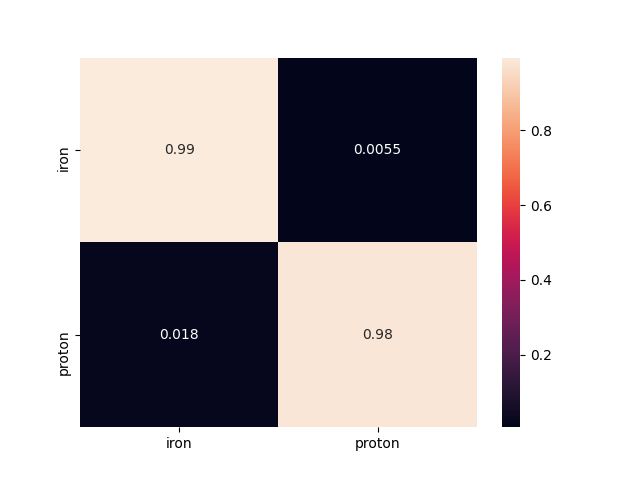
\includegraphics[width=.8\linewidth]{imagenes/06_Experimentacion/caecm.png}  
  \caption{CAE confusion matrix.}
  \label{fig:caecm}
\end{subfigure}

\newline

\begin{subfigure}{.5\textwidth}
  \centering
  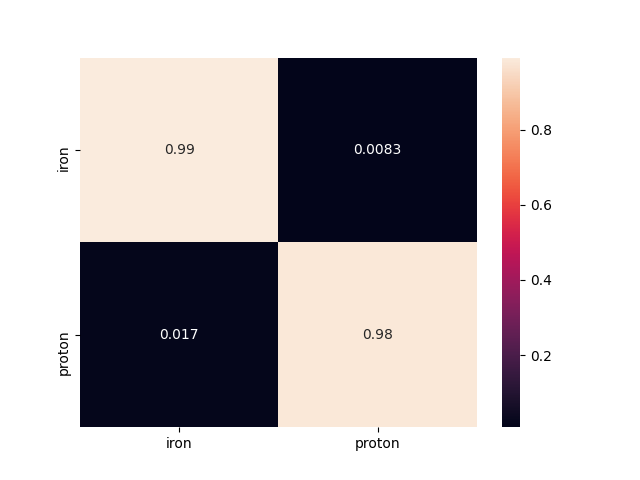
\includegraphics[width=.8\linewidth]{imagenes/06_Experimentacion/resnetcm.png}  
  \caption{ResNet confusion matrix.}
  \label{fig:resnetcm}
\end{subfigure}
\begin{subfigure}{.5\textwidth}
  \centering
  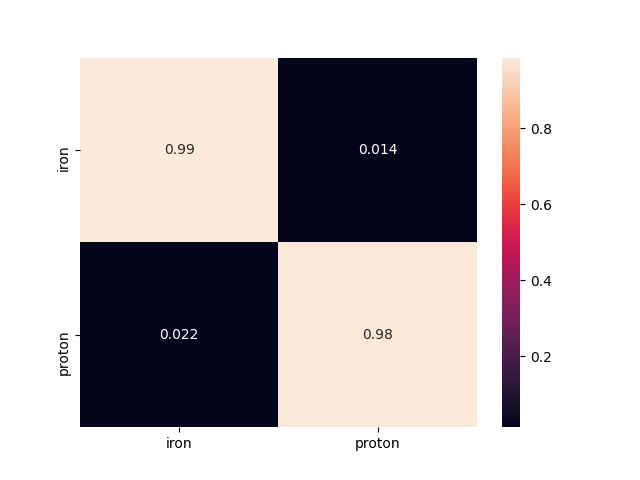
\includegraphics[width=.8\linewidth]{imagenes/06_Experimentacion/vaecm.png}  
  \caption{VAE confusion matrix.}
  \label{fig:vaecm}
\end{subfigure}
\caption{\textit{Confusion matrices} de los mejores resultados de los experimentos.}
\label{fig:confusion}
\end{figure}

\begin{table}[H]
\centering
\begin{tabular}{ccc}
\hline
\textbf{Experimento} &
  \textbf{Hiperparámetros} &
  \textbf{$\mathbf{F_1}$ score (Test)} \\ \hline
CAE &
  \begin{tabular}[c]{@{}c@{}}depth: 3\\ latent\_size: 65\\ batch\_size: 255\\ optimizer: adam\\ first\_conv\_out\_channels: 9\\ lr: 0.0029064860639852596\\ reg: 0.008171626239529795\end{tabular} &
  0.988 \\ \hline
Simple CNN &
  \begin{tabular}[c]{@{}c@{}}batch\_size: 180\\ optimizer: adam\\ out\_channels: {[}14, 18{]}\\ lr: 0.0017701827211672693\end{tabular} &
  0.991 \\ \hline
ResNet &
  \begin{tabular}[c]{@{}c@{}}batch\_size: 89\\ optimizer: sgd\\ lr: 0.0037730724227855905\\ reg: 0.0002618785645692275\\ number\_of\_blocks: {[}4, 6, 6, 5{]}\\ num\_channels: {[}14, 45, 86, 181, 430{]}\end{tabular} &
  0.987 \\ \hline
VAE &
  \begin{tabular}[c]{@{}c@{}}batch\_size: 37\\ optimizer: adam\\ lr: 0.0004440804594397368\\ reg: 0.0004545588488375805\end{tabular} &
  0.982 \\ \hline
\end{tabular}
\caption{Resultados de cada experimento}
\label{tab:results}
\end{table}

\newpage
\subsection{Análisis resultados \textit{Convolutional Autoencoder}}

\begin{figure}[H]
\begin{subfigure}{.5\textwidth}
  \centering
  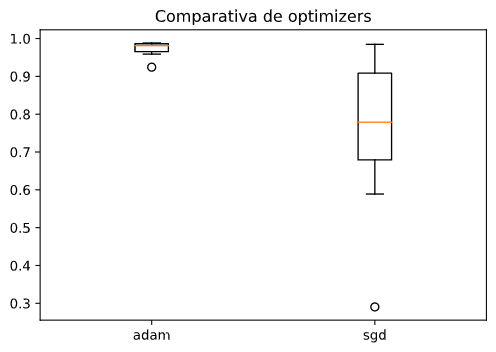
\includegraphics[width=.8\linewidth]{imagenes/06_Experimentacion/caeimages/caeoptimizers.png}
  \caption{\textit{Optimizers boxplot}.}
  \label{fig:caeoptimizers}
\end{subfigure}
\begin{subfigure}{.5\textwidth}
  \centering
  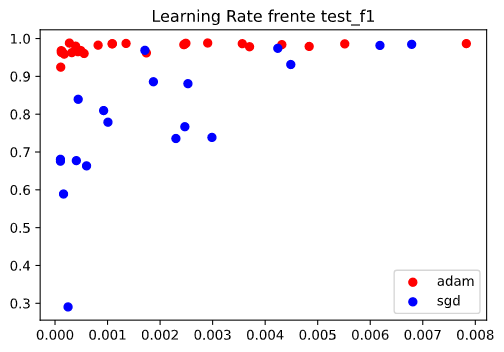
\includegraphics[width=.8\linewidth]{imagenes/06_Experimentacion/caeimages/caelr.png}  
  \caption{\textit{Learning rate} frente \textit{$F_1$ score}.}
  \label{fig:caelr}
\end{subfigure}

\newline

\begin{subfigure}{.5\textwidth}
  \centering
  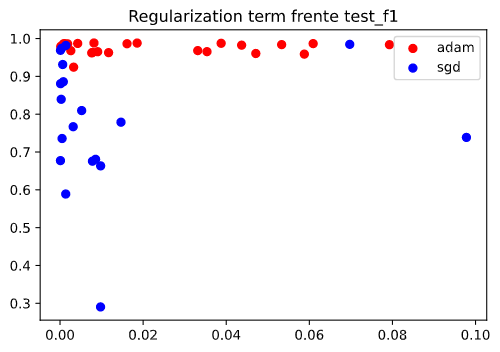
\includegraphics[width=.8\linewidth]{imagenes/06_Experimentacion/caeimages/caereg.png}
  \caption{\textit{Regularization} frente \textit{$F_1$ score}.}
  \label{fig:caeoreg}
\end{subfigure}
\begin{subfigure}{.5\textwidth}
  \centering
  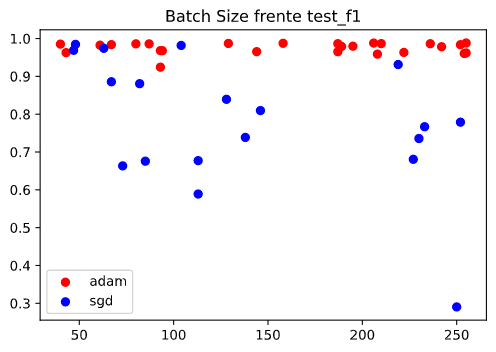
\includegraphics[width=.8\linewidth]{imagenes/06_Experimentacion/caeimages/caebs.png}  
  \caption{\textit{Batch size} frente \textit{$F_1$ score}.}
  \label{fig:caebr}
\end{subfigure}

\newline

\begin{subfigure}{.5\textwidth}
  \centering
  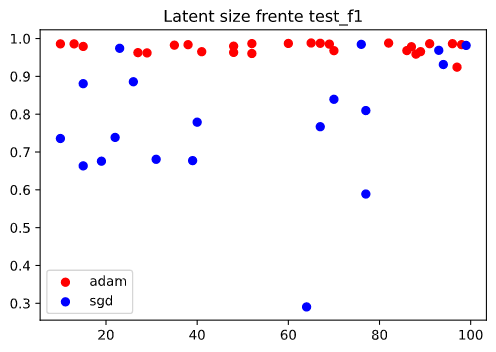
\includegraphics[width=.8\linewidth]{imagenes/06_Experimentacion/caeimages/caelatentsize.png}
  \caption{\textit{Latent Size} frente \textit{$F_1$ score}.}
  \label{fig:caelatentsize}
\end{subfigure}
\begin{subfigure}{.5\textwidth}
  \centering
  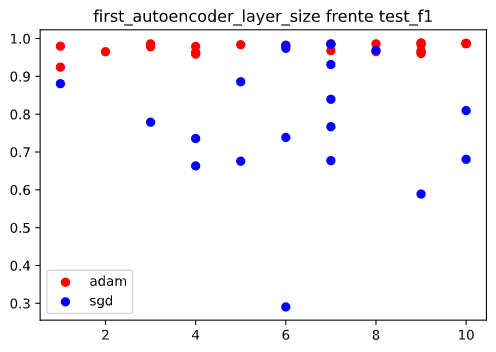
\includegraphics[width=.8\linewidth]{imagenes/06_Experimentacion/caeimages/caefcoc.png}  
  \caption{\textit{first\_autoencoder\_layer\_size} frente \textit{$F_1$ score}.}
  \label{fig:caefcoc}
\end{subfigure}

\caption{Plots para analizar del efecto de los hiperparámetros en los resultados del experimento CAE.}
\label{fig:caeanalysis}
\end{figure}

Viendo la Figura \ref{fig:caeanalysis} podemos sacar las siguientes conclusiones:

\begin{itemize}
    \item De la Figura \ref{fig:caeoptimizers} podemos sacar como conclusión que el optimizador \textit{Adam} da mejores resultados que \textit{SGD} por mucho. A parte de tener resultados mejores, estos son menos dispersos y están a la altura del Q4 de los resultados de \textit{SGD}.
    \item En la Figura \ref{fig:caelr} podemos observar que \textit{Adam} saca buenos resultados independientemente del valor del \textit{learning rate}. Sobre \textit{SGD}, parece que a más alto es el valor, mejores resultados saca (en la Figura \ref{fig:caesgdcorr} podemos observar una correlación positiva y alta).
    \item Sobre la Figura \ref{fig:caeoreg} podemos decir que el valor de la regularización no afecta mucho al resultado. De hecho, \textit{Adam} saca buenos resultados independientemente del valor de este hiperparámetro y en la Figura \ref{fig:caesgdcorr} podemos ver que no hay mucha correlación entre el valor de \textit{test\_f1} del resultado del optimizador \textit{SGD} y el \textit{lr}
    \item Parece haber una correlación negativa media entre el \textit{Bath Size} y el \textit{test\_f1} para el optimizador \textit{SGD}, por lo que más o menos podemos decir que a más pequeño sea el \textit{Bath Size}, mejor resultado obtendremos usando \textit{SGD}. Con \textit{Adam} siempre se obtiene buen resultado.
    \item Sobre los demás hiperparámetros, parece que no tienen mucho efecto sobre la capacidad de clasificación del modelo final.
\end{itemize}

\begin{figure}[H]
  \centering
  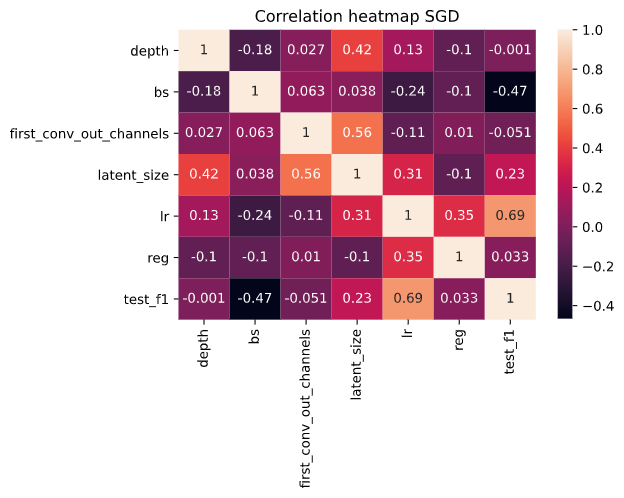
\includegraphics[width=.8\linewidth]{imagenes/06_Experimentacion/caeimages/caesgdcorr.png}  
  \caption{Correlación entre los hiperparámetros y \textit{test\_f1} para los resultados del optimizador \textit{SGD} (experimento CAE).}
  \label{fig:caesgdcorr}
\end{figure}

\subsection{Análisis resultados \textit{Convolutional Classifier}}

\begin{figure}[H]
\begin{subfigure}[b]{.5\textwidth}
  \centering
  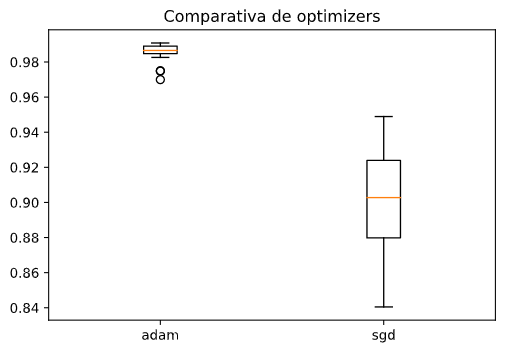
\includegraphics[width=.8\linewidth]{imagenes/06_Experimentacion/simplecnn/simplecnnboxplot.png}
  \caption{\textit{Optimizers boxplot}.}
  \label{fig:simplecnnoptimizers}
\end{subfigure}
\begin{subfigure}[b]{.5\textwidth}
  \centering
  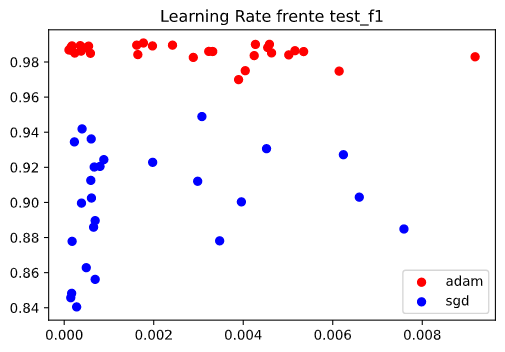
\includegraphics[width=.8\linewidth]{imagenes/06_Experimentacion/simplecnn/simplecnnlr.png}  
  \caption{\textit{Learning rate} frente \textit{$F_1$ score}.}
  \label{fig:simplecnnlr}
\end{subfigure}\\

\begin{subfigure}[b]{.5\textwidth}
  \centering
  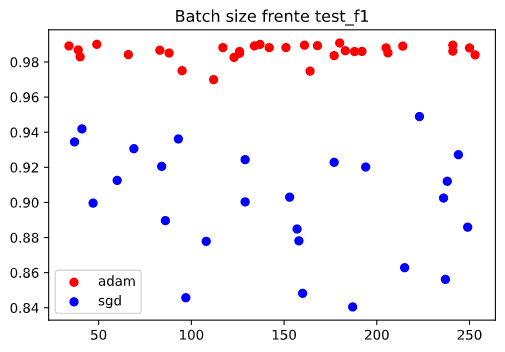
\includegraphics[width=.8\linewidth]{imagenes/06_Experimentacion/simplecnn/simplecnnbs.png}
  \caption{\textit{Batch Size} frente \textit{$F_1$ score}.}
  \label{fig:simplecnnreg}
\end{subfigure}

\caption{Plots para analizar del efecto de los hiperparámetros en los resultados del experimento Simple CNN.}
\label{fig:simplecnnanalysis}
\end{figure}

De los \textit{plots} de la Figura \ref{fig:simplecnnanalysis} podemos sacar las siguientes conclusiones:

\begin{itemize}
    \item De nuevo con \textit{Adam} se obtinen mejores resultados que con \textit{SGD}, pero esta vez la diferencia es mayor (esto se puede observar en la Figura \ref{fig:simplecnnoptimizers}).

    \item Con \textit{Adam} se obtienen buenos resultados independientemente del \textit{learning rate}. Sin embargo, con \textit{SGD} no hay mucha correlación entre el valor de este hiperparámetro y la métrica \textit{test\_f1} (esto se puede ver en la Figura \ref{fig:simplecnncorr}).
    
    \item Al igual que en el punto anterior, con \textit{Adam} también se obtienen buenos resultado independientemente del valor del \textit{batch size}. Con \textit{SGD} hay una correlación negativa baja entre este hiperparámetro y la métrica \textit{test\_f1} (ver Figura \ref{fig:simplecnncorr}).
\end{itemize}

\begin{figure}[H]
  \centering
  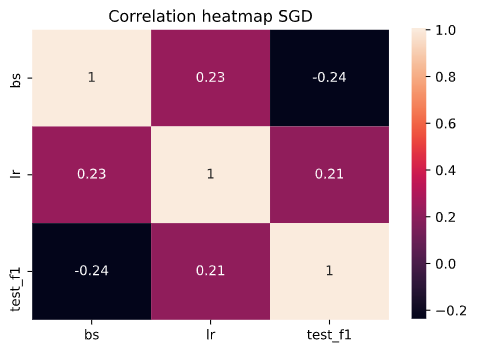
\includegraphics[width=.8\linewidth]{imagenes/06_Experimentacion/simplecnn/simplecnnsgdcorr.png}  
  \caption{Correlación entre los hiperparámetros y \textit{test\_f1} para los resultados del optimizador \textit{SGD} (experimento Simple CNN).}
  \label{fig:simplecnncorr}
\end{figure}

\subsection{Análisis resultados \textit{ResNet}}

\begin{figure}[H]
\begin{subfigure}[b]{.5\textwidth}
  \centering
  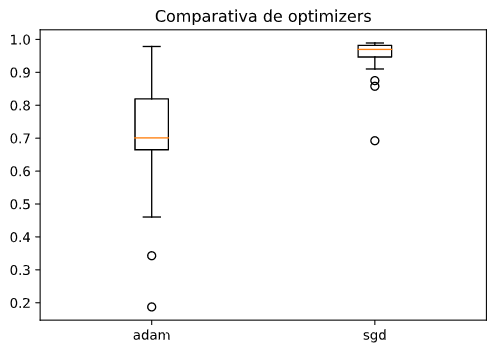
\includegraphics[width=.8\linewidth]{imagenes/06_Experimentacion/resnet/resnetboxplot.png}
  \caption{\textit{Optimizers boxplot}.}
  \label{fig:resnetoptimizers}
\end{subfigure}
\begin{subfigure}[b]{.5\textwidth}
  \centering
  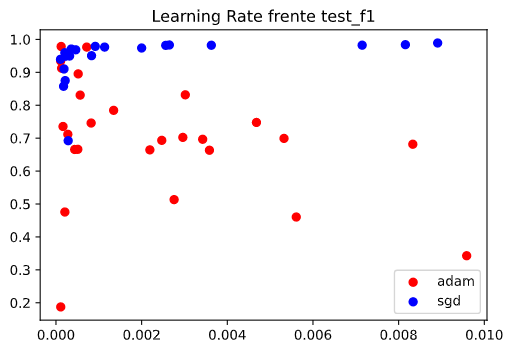
\includegraphics[width=.8\linewidth]{imagenes/06_Experimentacion/resnet/resnetlr.png}
  \caption{\textit{Learning rate} frente \textit{$F_1$ score}.}
  \label{fig:resnetlr}
\end{subfigure}\\

\begin{subfigure}[b]{.5\textwidth}
  \centering
  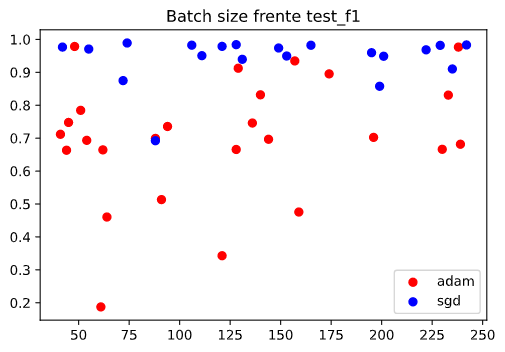
\includegraphics[width=.8\linewidth]{imagenes/06_Experimentacion/resnet/resnetbs.png}
  \caption{\textit{Batch Size} frente \textit{$F_1$ score}.}
  \label{fig:resnetbs}
\end{subfigure}
\begin{subfigure}[b]{.5\textwidth}
  \centering
  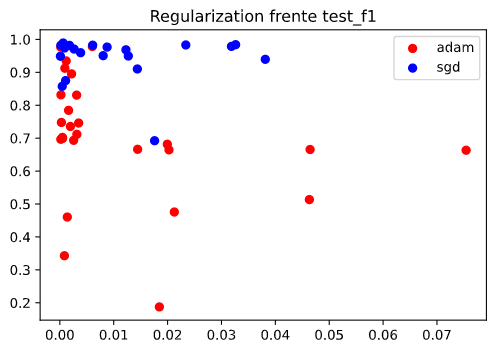
\includegraphics[width=.8\linewidth]{imagenes/06_Experimentacion/resnet/resnetreg.png}
  \caption{\textit{Regularization} frente \textit{$F_1$ score}.}
  \label{fig:resnetreg}
\end{subfigure}

\caption{Plots para analizar del efecto de los hiperparámetros en los resultados del experimento ResNet.}
\label{fig:resnetanalysis}
\end{figure}

De la Figura \ref{fig:resnetanalysis} podemos sacar las siguientes conclusiones:

\begin{itemize}
    \item Viendo la Figura \ref{fig:resnetoptimizers}, vemos que por primera vez \textit{SGD} saca mejores resultados que \textit{Adam} y por bastante (los resultados de \textit{SGD} están a la altura del Q4 de \textit{Adam} y la mediana es mucho más alta). De hecho, el mejor resultado para la métrica \textit{test\_f1} ha sido usando el optimizador \textit{SGD} (ver Tabla \ref{tab:results}).
    \item En la Figura \ref{fig:resnetlr} se puede observar que con el optimizador \textit{SGD} parece que se van obteniendo mejores resultados conforme se va aumentando el \textit{learning rate} aunque la correlación, que se puede ver en la Figura \ref{fig:resnetsgdcorr}, no es muy alta. En cambio, con \textit{Adam} parece que con un \textit{learning rate} alto va dando peores resultados, aunque la correlación (ver Figura \ref{fig:resnetadamcorr}) también es débil.
    \item Observando la Figura \ref{fig:resnetbs} parece no haber relación entre el \textit{Batch Size} y la métrica \textit{test\_f1}, de hecho la correlación es débil (ver Figura \ref{fig:resnetsgdcorr} y Figura \ref{fig:resnetadamcorr}).
    \item Viendo la Figura \ref{fig:resnetreg}, podemos confirmar que la regularización no tiene efecto notable en el resultado del optimizador \textit{SGD}. En el caso de \textit{Adam}, parece que el valor de regularización tampoco afecta demasiado al resultado.
\end{itemize}

\begin{figure}[H]
\begin{subfigure}[b]{.5\textwidth}
  \centering
  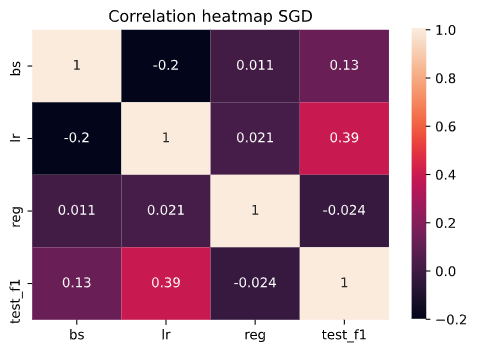
\includegraphics[width=.8\linewidth]{imagenes/06_Experimentacion/resnet/resnetsgdcorr.png}
  \caption{Correlación entre los hiperparámetros y \textit{test\_f1} para los resultados del optimizador \textit{SGD}.}
  \label{fig:resnetsgdcorr}
\end{subfigure}
\begin{subfigure}[b]{.5\textwidth}
  \centering
  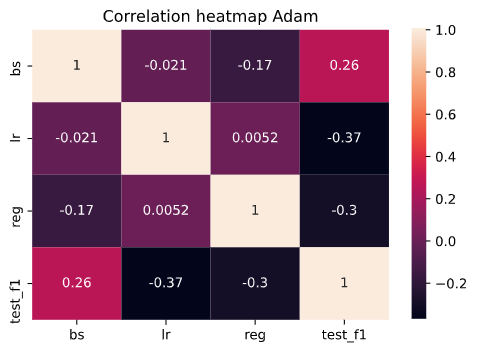
\includegraphics[width=.8\linewidth]{imagenes/06_Experimentacion/resnet/resnetadamcorr.png}
  \caption{Correlación entre los hiperparámetros y \textit{test\_f1} para los resultados del optimizador \textit{Adam}.}
  \label{fig:resnetadamcorr}
\end{subfigure}

\caption{Matrices de correlación entre los hiperparámetros y la métrica \textit{test\_f1} (experimento ResNet).}
\label{fig:resnetcorrelationmatrices}
\end{figure}

\subsection{Análisis de resultados \textit{Varitional Autoencoder}}

\begin{figure}[H]
\begin{subfigure}[b]{.5\textwidth}
  \centering
  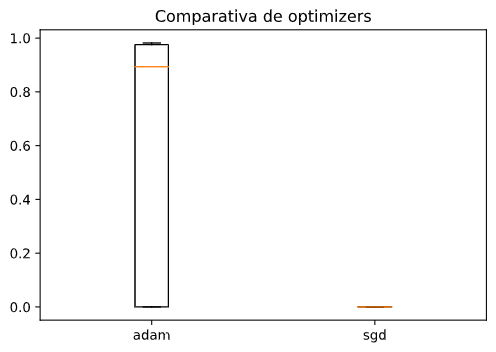
\includegraphics[width=.8\linewidth]{imagenes/06_Experimentacion/vae/vaeboxplot.png}
  \caption{\textit{Optimizers boxplot}.}
  \label{fig:vaeoptimizers}
\end{subfigure}
\begin{subfigure}[b]{.5\textwidth}
  \centering
  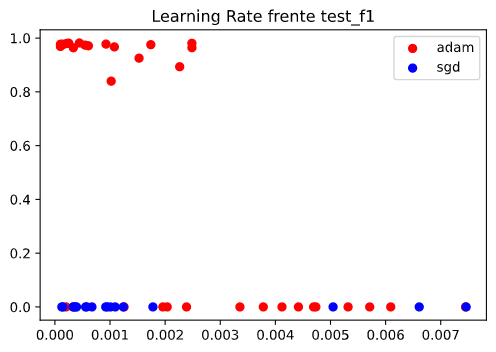
\includegraphics[width=.8\linewidth]{imagenes/06_Experimentacion/vae/vaelr.png}
  \caption{\textit{Learning rate} frente \textit{$F_1$ score}.}
  \label{fig:vaelr}
\end{subfigure}\\

\begin{subfigure}[b]{.5\textwidth}
  \centering
  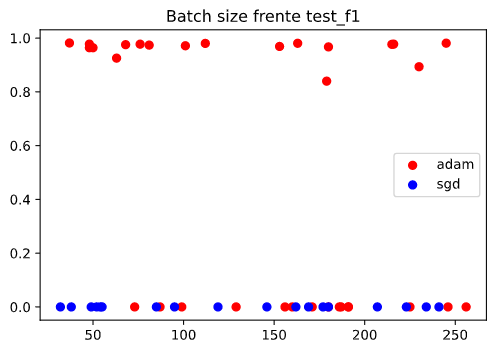
\includegraphics[width=.8\linewidth]{imagenes/06_Experimentacion/vae/vaebs.png}
  \caption{\textit{Batch Size} frente \textit{$F_1$ score}.}
  \label{fig:vaebs}
\end{subfigure}
\begin{subfigure}[b]{.5\textwidth}
  \centering
  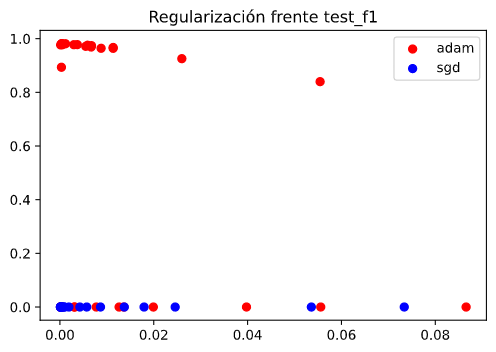
\includegraphics[width=.8\linewidth]{imagenes/06_Experimentacion/vae/vaereg.png}
  \caption{\textit{Regularization} frente \textit{$F_1$ score}.}
  \label{fig:vaereg}
\end{subfigure}

\caption{Plots para analizar del efecto de los hiperparámetros en los resultados del experimento VAE.}
\label{fig:vaeanalysis}
\end{figure}

De la Figura \ref{fig:resnetanalysis} podemos extraer las siguientes conclusiones:

\begin{itemize}
    \item Como se puede ver en la Figura \ref{fig:vaeoptimizers}, con \textit{SGD} no podemos entrenar un modelo que sea capaz de predecir, solo podemos usar \textit{Adam} para obtener unos resultados aceptables. Por tanto, en los siguientes puntos solo hablaré sobre los resultados obtenidos con este optimizador.
    \item Sobre el \textit{learning rate}, si es mayor que 0.003 es imposible obtener buenos resultados (como se puede ver en la Figura \ref{fig:vaelr}). Además, en la Figura \ref{fig:vaecorr} que hay una correlación negativa fuerte entre \textit{lr} y \textit{test\_f1}, confirmando mi afirmación.
    \item El \textit{Batch Size} no parece influir mucho en la métrica resultante, parece que al aumentar el valor es probable que de peor resultado como se puede ver en la Figura \ref{fig:vaebs} y en la Figura \ref{fig:vaecorr} se puede observer una correlación débil negativa.
    \item Viendo la Figura \ref{fig:vaereg} casi se puede afirmar que al aumentar el valor de la regularización, se va empeorando también el valor de la métrica \textit{test\_f1}.
\end{itemize}

\begin{figure}[H]
  \centering
  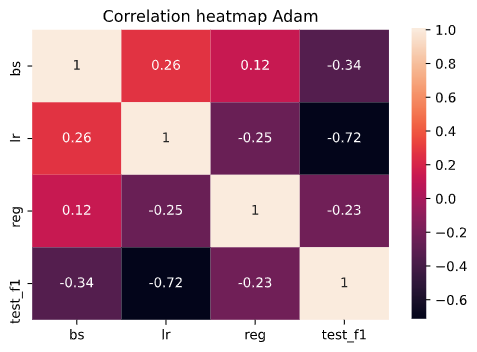
\includegraphics[width=.8\linewidth]{imagenes/06_Experimentacion/vae/vaeadamcorr.png} 
  \caption{Correlación entre los hiperparámetros y \textit{test\_f1} para los resultados del optimizador \textit{Adam} (experimento VAE).}
  \label{fig:vaecorr}
\end{figure}

\subsection{Análisis del uso de normalización}

Esta subsección ha sido añadida debido a un descuido que tuve (se me olvidó probar los resultados con los datos sin normalizar y normalizados para comparar resultados). En cuanto al análisis del efecto de la normalización, viendo los \textit{plots} de la Figura \ref{fig:normalization} podemos sacar las siguientes conclusiones:

\begin{itemize}
    \item Primeramente, en la Figura \ref{fig:caenorm} podemos ver que para el \textit{Convolutional Autoencoder} el uso de normalización empeora los resultados un poco para el caso del optimizador \textit{Adam} y bastante para el caso del optimizador \textit{SGD}.
    \item Para el caso de \textit{ResNet}, como se puede ver en la Figura \ref{fig:resnetnorm}, los resultados del \textit{SGD} mejoran un poco (el limite inferior de Q1 está más alto y el límite superior del Q4 está un poco más alto), pero se empeoran para \textit{Adam}.
    \item Para el caso de \textit{ConvClassifier} (ver Figura \ref{fig:simplecnnnorm}) y usando el optimizador \textit{SGD}, se obtienen mejores resultados sin regularización, pues la mediana está más alta y también el límite inferior de Q1 y el límite superior de Q4. Con el optimizador \textit{Adam}, parece que también se obtienen mejores resultados sin usar normalización, aunque la mediana esté más alta cuando se usa regularización, el límite superior de Q4 está más alto cuando no se usa regularización.
    \item Por último, con el modelo \textit{Varitional Autoencoder} (ver Figura \ref{fig:vaenorm}), los resultados con \textit{SGD} son claramente mejores cuando se usa normalización. En cuanto a \textit{Adam}, los resultados son mucho peores cuando se usa normalización.
\end{itemize}

\begin{figure}[H]
\begin{subfigure}{.5\textwidth}
  \centering
  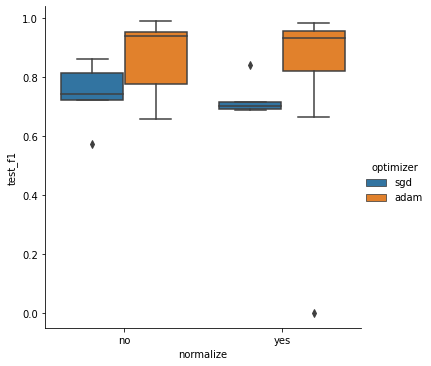
\includegraphics[width=.8\linewidth]{imagenes/06_Experimentacion/normalization/caenorm.png}  
  \caption{\textit{Plot} para análisis del efecto de la normalización en el modelo CAE.}
  \label{fig:caenorm}
\end{subfigure}
\begin{subfigure}{.5\textwidth}
  \centering
  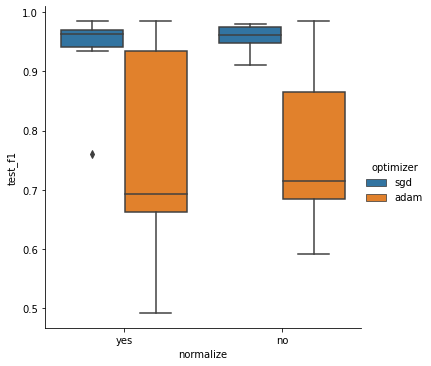
\includegraphics[width=.8\linewidth]{imagenes/06_Experimentacion/normalization/resnetnorm.png}  
  \caption{\textit{Plot} para análisis del efecto de la normalización en el modelo ResNet.}
  \label{fig:resnetnorm}
\end{subfigure}

\newline

\begin{subfigure}{.5\textwidth}
  \centering
  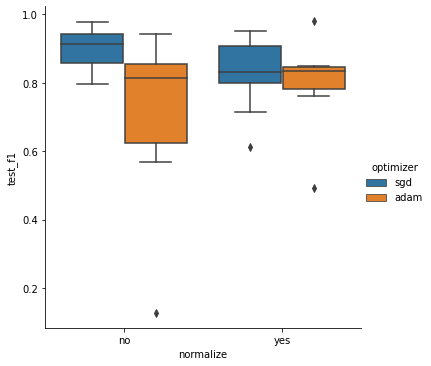
\includegraphics[width=.8\linewidth]{imagenes/06_Experimentacion/normalization/simplecnnnorm.png}  
  \caption{\textit{Plot} para análisis del efecto de la normalización en el modelo SimpleCNN.}
  \label{fig:simplecnnnorm}
\end{subfigure}
\begin{subfigure}{.5\textwidth}
  \centering
  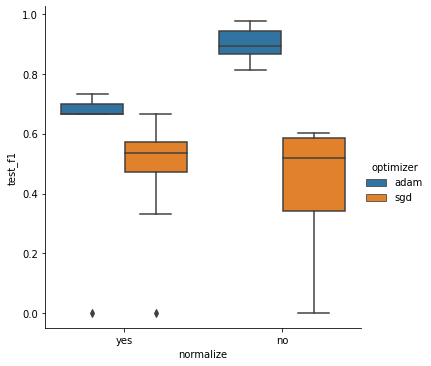
\includegraphics[width=.8\linewidth]{imagenes/06_Experimentacion/normalization/vaenorm.png}  
  \caption{\textit{Plot} para análisis del efecto de la normalización en el modelo VAE.}
  \label{fig:vaenorm}
\end{subfigure}
\caption{\textit{Plots} para análisis del efecto de la normalización.}
\label{fig:normalization}
\end{figure}
